% Awesome CV LaTeX Template
%
% This template has been downloaded from:
% https://github.com/huajh/huajh-awesome-latex-cv
%
% Author:
% Junhao Hua


%Section: Work Experience at the top
\sectionTitle{Recent Projects}{\faCode}

\begin{experiences}

    \experience
    {Jul 2019} {Custom Audiometry}{ITS}{C/Python}
	{Oct 2023} {
        \begin{itemize}
            \item Project owner: Dr. Dhany Arifianto, S.T, M.Eng, Ph.D
            \item Funded by: LPDP Rispro Invitation
            \item Company Partner: PT Xirca Dama Persada.
            \item Implementing \textit{3-Force Choice} Hearing Test in simple console
	        \item Built on STM32F401RE or STM32F303RB equipped with MAX98357A audio chip
    	    \item OLED Display and HTTPS Data exchange using ESP32 controller
            \item Patent Submission: \link{https://pdki-indonesia.dgip.go.id/detail/d420f8e76077ce4b84f4d3caafccce132c5f2e203691c5f0cc7db86c85b1ec95?nomor=P00202110888?nomor=P00202110888\&type=patent\&keyword=audiometer} {PDKI Database}
	        \item \faGithub: \link{https://github.com/VibrasticLab/pikoakustik2} {VibrasticLab/pikoakustik2}
            \item Prototype: 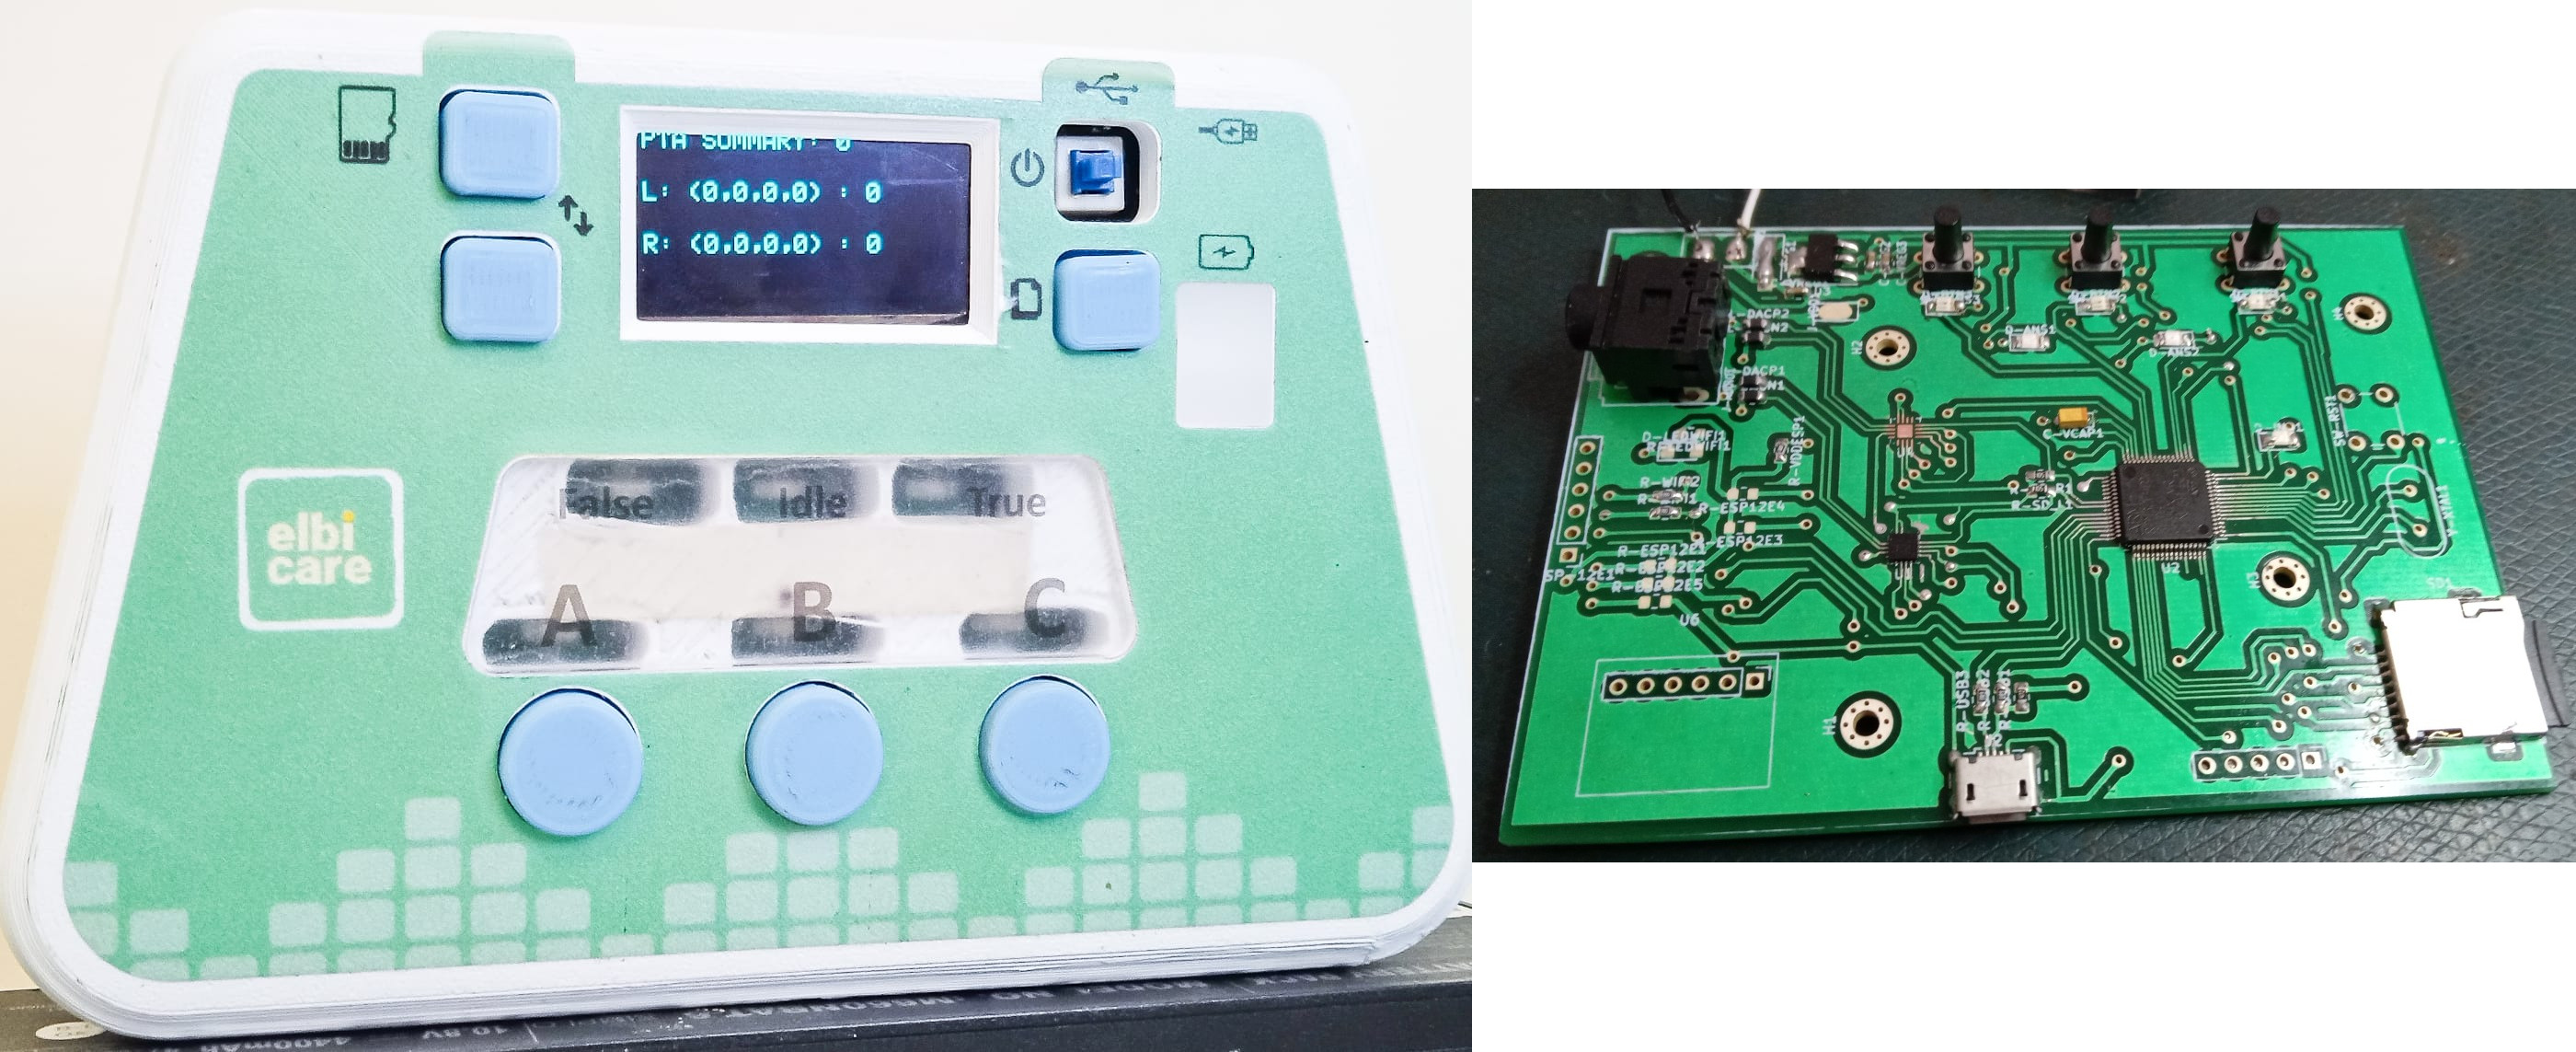
\includegraphics[width=0.4\textwidth]{images/audiometry.jpg}
        \end{itemize}
    }
    {KiCAD, STM32, C, Python, Audiometry, Medical Device, IoT}

    \emptySeparator
	\experience
    {Jun 2020} {Custom Cough Analyzer}{ITS}{C/Python}
	{Sept 2020} {
	\begin{itemize}
            \item Project owner: Dr. Dhany Arifianto, S.T, M.Eng, Ph.D
            \item Funded by: BRIN RIIM
	        \item Implementing Audio Processing using AI (Tensorflow)
	        \item Audio Capturing using RaspberryPi-4 equipped with INMP441 Microphone
	        \item \faGithub: \link{https://github.com/VibrasticLab/ehealth-iot} {VibrasticLab/ehealth-iot}
	        \item \faGithub: \link{https://github.com/VibrasticLab/ehealth-web} {VibrasticLab/ehealth-web}
            \item Prototype: 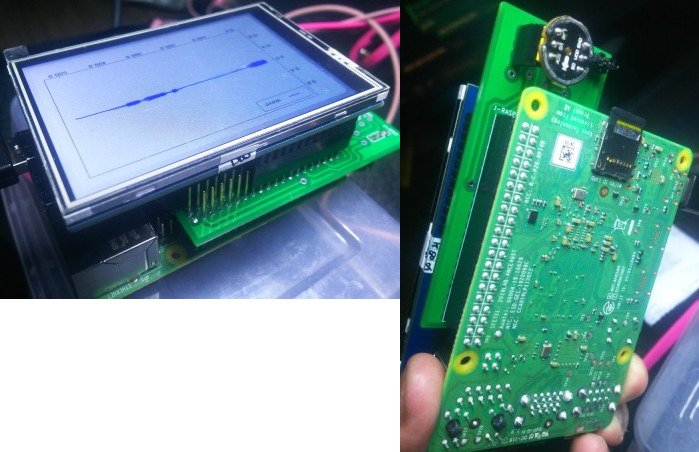
\includegraphics[width=0.4\textwidth]{images/cough.jpg}
	\end{itemize}
    }
    {KiCAD, RaspberryPi, C, Python, Cough, Medical Device, IoT, Web, AI}

    \emptySeparator
	\experience
    {Aug 2022} {Vibration Monitor}{ITS}{C/Python}
	{Jun 2023} {
	\begin{itemize}
            \item Project owner: Dr. Dhany Arifianto, S.T, M.Eng, Ph.D
            \item Funded by: ITS Internal Funds
            \item Intended to be used in Railways as Condition Monitoring through LoRA Network
	        \item Implementing Vibration Monitoring based on STM32F051RB and TE-830-M1 sensor
	        \item Monitoring Vibrations and displayed on a PyQt interface through Serial Communication
	    \item \faGithub: \link{https://github.com/VibrasticLab/wesel\_monitoring} {VibrasticLab/wesel\_monitoring}
        \item Prototype: 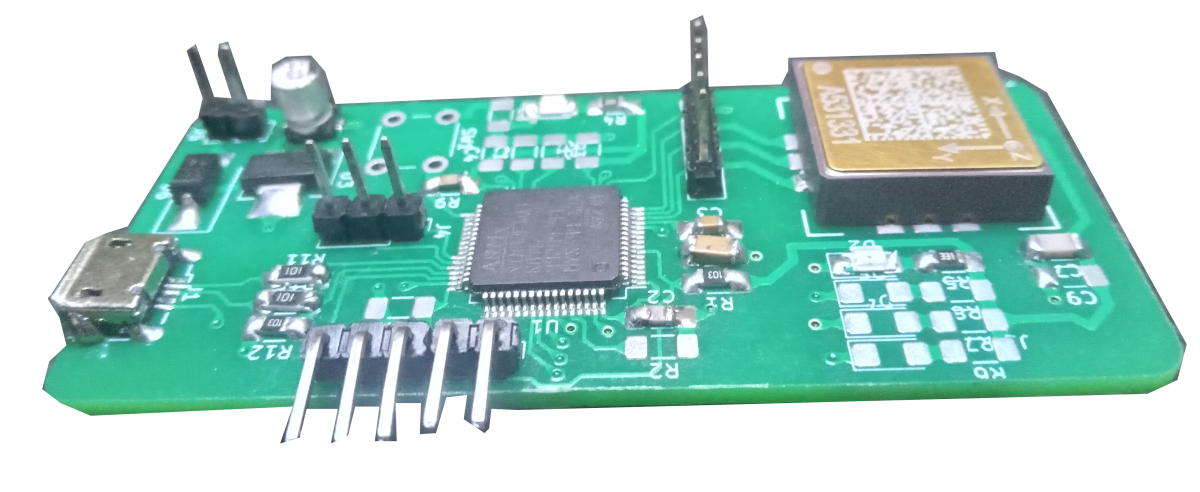
\includegraphics[width=0.4\textwidth]{images/vibs.png}
	\end{itemize}
    }
    {KiCAD, STM32, C, Python, Vibration, Serial, IoT}

    \emptySeparator
    \experience
    {Sept 2022} {Custom Engine Control}{PoltekMadiun}{C/C++}
    {Oct 2023} {
        \begin{itemize}
            \item Project owner: Deni Nur Fauzi, S.T, M.T
            \item Funded by: PoltekMadiun
            \item Implementing Control Unit for Custom Engine
            \item Built on STM32F051RB, read engine's crankshaft to control sparkplug timing
            \item \faGithub: \link{https://github.com/deninur2427/ecu\_pnm} {ecu\_pnm}
            \item Prototype: 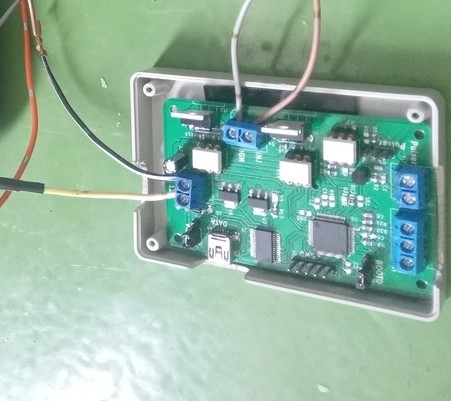
\includegraphics[width=0.4\textwidth]{images/ecu_pnm.jpg}
        \end{itemize}
    }
    {KiCAD, STM32, C, C++, Engine Control, Serial Interfacing, IoT}


\end{experiences}
